\documentclass{article}
\usepackage[usenames,dvipsnames]{xcolor}
\usepackage{palatino}
\usepackage{amsmath}
\usepackage[utf8]{inputenc}
\usepackage[T1]{fontenc}
\usepackage{amssymb}
\usepackage[colorlinks=true]{hyperref}
\usepackage{tikz}
\usepackage{graphicx}
%\usepackage[margin=1in]{geometry}
\usepackage{listings}

\newcommand{\hshim}{2.0cm}
\newcommand{\vshim}{-1cm}

\newcommand{\dtwo}[2]{\parbox[s]{3.5cm}{\colorbox{green}{#1}  \newline\ \colorbox{green}{#2}}}
\newcommand{\done}[1]{\parbox[s]{3.5cm}{\colorbox{green}{#1}}}
\newcommand{\sone}[1]{\parbox[s]{3.5cm}{\colorbox{pink}{#1}}}
\newcommand{\skkp}[2]{\parbox[s]{3.5cm}{\colorbox{pink}{#1} \newline\ \colorbox{pink}{#2}}}
\newcommand{\tone}[1]{\parbox[s]{3.5cm}{\colorbox{yellow}{#1}}}
\newcommand{\todo}[2]{\parbox[s]{3.5cm}{\colorbox{yellow}{#1} \newline\ \colorbox{yellow}{#2}}}

\newcommand{\colorcode}{{\hfill \colorbox{yellow}{\vphantom{X}}~~TODO \hfill \colorbox{pink}{\vphantom{X}}~~Skipped \hfill \colorbox{green}{\vphantom{X}}~~Done \hfill}}

\renewcommand{\maketitle}{{%
\flushleft{Ben Greenman \hfill \today} \\
{CS 7485 : Wrap-up \hfill Kodkod $\sqrt{2}$} \\
\vspace{1mm}
\hrule
\vspace{0.4cm}}}

\newcommand{\secref}[1]{Section~\ref{#1}}
\newcommand{\figref}[1]{Figure~\ref{#1}}

\lstdefinelanguage{Scheme}{
    morekeywords=[1]{define, define-syntax, define-macro, lambda, define-stream, stream-lambda},
        morekeywords=[2]{begin, call-with-current-continuation, call/cc,
            call-with-input-file, call-with-output-file, case, cond,
            do, else, for-each, if,
                let*, let, let-syntax, letrec, letrec-syntax,
                    let-values, let*-values,
                    and, or, not, delay, force,
                    quasiquote, quote, unquote, unquote-splicing,
                    map, fold, syntax, syntax-rules, eval, environment, query },
        morekeywords=[3]{import, export},
        alsodigit=!\$\%&*+-./:<=>?@^_~,
        sensitive=true,
        morecomment=[l]{;},
        morecomment=[s]{\#|}{|\#},
        morestring=[b]",
        basicstyle=\small\ttfamily,
        keywordstyle=\bf\ttfamily\color[rgb]{0,.3,.7},
        commentstyle=\color[rgb]{0.133,0.545,0.133},
        stringstyle={\color[rgb]{0.75,0.49,0.07}},
        upquote=true,
        breaklines=true,
        breakatwhitespace=true,
        literate=*{`}{{`}}{1}
}
\lstset{
  language=Scheme,
  showstringspaces=false,
  inputencoding=utf8,
  extendedchars=true
}

\begin{document}
\maketitle

\begin{abstract}
  The goal of my \href{http://www.ccs.neu.edu/home/wahl/Teaching/Software-Model-Checking/2016-Spring/}{CS 7485} course project was to port the \href{http://alloy.mit.edu/kodkod/}{Kodkod} relational logic solver from Java to Racket
   and compare the two implementations.
  This is an end-of-semester status report: I was unable to meet the original
   goal but have implemented a Kodkod-inspired compiler from propositional
   logic to CNF (\secref{sec:compile}) and run some very simple benchmarks (\secref{sec:eval}).
  Remaining goals are listed in \secref{sec:future}.
\end{abstract}

\section{Motivation}
\label{sec:motivation}

The \href{https://emina.github.io/rosette/}{Rosette} solver-aided language
 is an interesting research project aimed at spanning a gap between formal
 methods and programming.
Rosette's goal is to help programming language designers incorporate
 SMT and/or SAT solver technology in domain-specific programming languages (DSLs).
It does so by implementing a compiler from a high-level language (suitable
 for general purpose programming or for designing DSLs) to solver formulas.

Until recently, Rosette gave users the choice of three solver backends:
 Microsoft's \href{https://github.com/Z3Prover/z3/wiki}{Z3} solver,
 NYU's \href{http://cvc4.cs.nyu.edu/web/}{CVC4},
 and MIT's \href{http://alloy.mit.edu/kodkod/index.html}{Kodkod} solver.
Kodkod was the default backend and Kodkod is implemented in Java.
So new Rosette users had to first install Racket\footnote{Rosette is implemented in Racket.}
 and then install Java before they could begin using Rosette's solver-aided languages.

My goal was to move the Java implementation to Racket, with the hope that
 all of Rosette could be implemented in a single language.
As a secondary goal, I wanted to learn how to implement a model checker
 and at least ``go through the motions'' of writing one.\footnote{Hunter S. Thompson used to ``go through the motions'' of writing a great novel by copying pages from \emph{The Great Gatsby}~\cite{ny}. There are worse role models.}

Of these three goals, only 1 was really successful:
 I learned plenty about how Kodkod is implemented.
But I have much more to learn, because to date I have only written a compiler from
 propositional logic to CNF.
Hence the revised name of this semester project: Kodkod $\sqrt{2}$.
One checkpoint has been implemented, but the road to completing the solver
 stretched on far longer than I expected, and seemed to increase the more I
 learned.

The reason my second goal of implementing all Rosette in Racket has failed is
 due to a technicality.
Kodkod is designed to use a \emph{fast} external SAT solver and all the best
 are written in C.



\section{Kodkod Architecture}
\label{sec:kodkod}

Kodkod was designed and implemented by Emina Torlak as part of her PhD thesis
 under Daniel Jackson at MIT~\cite{t-dissertation-2009}.
Her thesis and \href{http://alloy.mit.edu/kodkod/release/current/doc/}{Java implemention} were the primary guides for my work.

Kodkod is a solver for relational logic designed to effectively utilize partial solutions.
Relational logic is first-order logic extended with a handful of so-called relational operators
 to express properties like the transpose and closure of bounded variables.
%\begin{itemize}
%\item $\sim e$ is the transpose of the expression $e$
%\item $\hat{}e$ is the transitive closure of $e$
%\item $* e$ is the reflexive closure of $e$
%\end{itemize}
There are three key assumptions supporting Kodkod's design:
\begin{itemize}
\item Relational logic is well-suited for describing engineering problems.
   For instance, transitive closure can describe reachability in a graph.
\item Engineers often have access to partial solutions, informations from
   which should be used the guide the search for a full solution.
\item Modern SAT solvers are extremely fast, to the point that compiling
   a high-level logic to SAT queries is competitive with compiling to SMT.
\end{itemize}

We assume these are still valid, but it would be interesting to compare
 today's SAT and SMT solvers and perhaps reproduce the earlier results that
 SAT was arguably the better choice.

The high-level architecture of Kodkod is show in \figref{fig:arch}.
Input from the user, represented on the left of the figure, comes in three
 required forms.
First is a listing of the \emph{atoms} over which the problem and its solutions
 will be expressed.
These are a finite set of otherwise arbitrary symbols.
Second are \emph{relational bounds} expressed in terms of the atoms.
Each relational bound is an identifier {\tt ID} and two sets of tuples of atoms\textemdash
 in other words, two relations on atoms.
The first relation is a lower bound and expresses the relations that must
 be included in {\tt ID}.
The second relation is an upper bound and expresses relations that might be
 in {\tt ID}.
The lower and upper bounds must contain tuples of the same arity.
Also the lower bound must be contained in the upper bound.
For example, given the atoms {\tt\{true, false\}}
 the type {\tt Boolean} can be encoded by giving {\tt\{(true, false)\}} as
 both the upper and lower bound.
Third are formulas over the atoms and variables written in relational logic.
These formulas may be constraints in the problem or partial solutions.

The second phase of Kodkod, shown in the middle of the figure, is a translation
 from relational logic to an intermediate representation of boolean matrices.
First existential variables are Skolemized up to a user-determined depth.
Then relations $R$ over the $N$ atoms of the problem are encoded as $N \times N$
 matrices where the entry at row $i$ and column $j$ is 1 iff the pair of atoms
 $(i, j)$ is in the relation $R$.
Similarly, relational bounds of arity $k$ are encoded as $k$-dimensional matrices
 using boolean variables as unknowns.

Two important optimizations occur at this stage.
First, the matrices are represented sparsely because most relations in a problem
 deal with only a few atoms.
Second, matrices are compacted using a technique by Torlak~\cite{t-dissertation-2009}
 for detecting symmetries and sharing data.

After a problem is converted to a compact boolean form, it is compiled to a boolean
 circuit and then translated to CNF for a solver.
The data is then fed to an off-the-shelf SAT solver.
If the solver proves the formula, all is well.
If not, we use a final key ingredient of Kodkod: minimal core extraction.
From the solver's proof of unsatisfiability Kodkod infers a minimal counterexample
 to the specification and presents it to the user.
In practice, this makes using the solver must less frustrating.

\begin{figure}
  \label{fig:arch}
  \begin{center}
  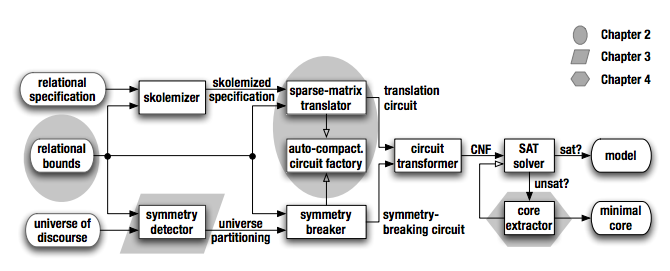
\includegraphics[width=12cm]{arch.png}
  \end{center}
  \caption{Kodkod architecture}
\end{figure}



\section{Implementation}
\label{sec:compile}

The implementation for my semester project is hosted on \href{https://github.com/bennn/rkt-kodkod}{Github}.
Currently the implementation is 2,500 lines of Racket code and implements a compiler from \emph{propositional} logic to CNF.

\begin{figure}
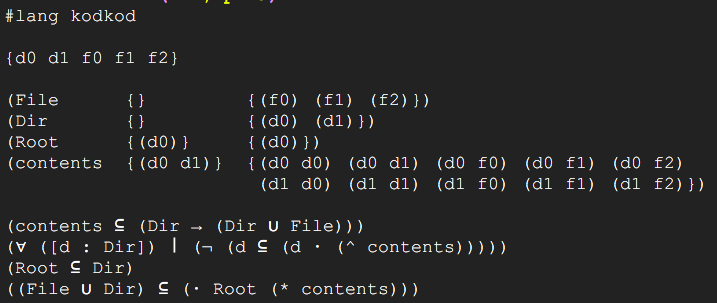
\includegraphics[width=10cm]{rkt.png}

  \vspace{0.1cm}
  %\hrule
  \hrule\hrule
  %\vspace{0.1cm}

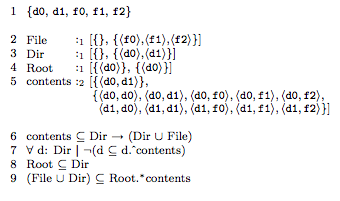
\includegraphics[width=10cm]{fs.png}
\caption{Racket code vs. mathematical specification}
\label{fig:lang}
\end{figure}

The surface syntax (\figref{fig:lang}) directly follows the formal syntax of relational logic.
Logic problems are written naturally with sets for atoms \& bounds and
 unicode for logical operators.
Typographical errors in the problem spec are reported in terms of source code
 lines and positions.

After reading a file into a data structure representing a relational logic
 formula, we compile the formula to a boolean matrix representation.
Like Kodkod, this matrix is implemented sparsely.
We do not, however, have a skolemizer or symmetry detector.
Instead matrices are compiled na\"ively, with only the most obvious short-circuit
 optimizations.

Once the problem is translated to a matrix, we compile a boolean circuit and
 then translate the circuit to CNF.
The circuits do as much collapsing as is possible; for many formulas
 we can output SAT or UNSAT at this stage without calling an external solver,
 so this is where the project ends for the moment.


\subsection{Challenges}

The most difficult part of the project was choosing what to implement to
 reach deliverable checkpoints.
I did poorly at this task.
Reading the dissertation was informative, but focused primarily on Kodkod's
 technical contributions rather than on the details needed to walk a complete
 path from specification to SAT/UNSAT.
For example, I initially misunderstood that the boolean matrix representation
 is only for expressions and relational bounds, but \emph{not} for top-level
 formulas and constraints.
It was only after implementing most of an interpreter that I realized the dead-end.

Unfortunately the Java code was even worse to read due to a very high signal-to-noise
 ratio.
Kodkod is full of factories and generic class hierarchies that tend to obsure
 the purpose of each component, at least to someone unaccustomed to reading
 Java code.\footnote{Maybe my biggest problem was refusing to use an IDE like Eclipse or IntelliJ.}
There were also many diversions in the name of ease and optimization\textemdash
 rather than puzzle over the big picture of the code, it was easier to latch
 on to a data structure like the sparse-sequence-backed matrices and their
 supporting red-black tree data structure.
Implementing these was fun and interesting to think about how best to translate
 from Java, but ultimately did little to advance my goal of porting the Kodkod solver.


\subsection{Comparisons}

Some benefits of the rewrite over the original:
\begin{itemize}
\item The mathematical front-end syntax is much easier to use (and program)
 than Kodkod's Java API.
\item Racket's pattern-matching and variable-arity functions
 are concise alternatives to visitor and factory patterns.
\item Stateful, object-based data structures are almost all replaced with
 functional versions.
 Though, I have not benchmarked to see if this gave a performance improvement.
\end{itemize}


\section{Evaluation}
\label{sec:eval}

\figref{fig:bench} shows the results of a small experiment measuring the compile
 time of our implementation.
The code used the run the experiment and generate the figure is
 included in the appendix.

For each integer $N$ between 4 and 200 inclusive, we generated 20 random
 Kodkod programs and measured the time to complete a system call that invoked
 our compiler on the generated file.
Each green dot is the time for a single generated program.
The distribution is oddly bimodal, but even the worse trend is not bad\textemdash
 compile times run in less than 1 second and appear to scale linearly as programs
 grow in size.

To be precise, each $N$ generates a program with $N$ atoms, $N$ relational bounds,
 and $N$ binary formulas.
The lower and upper bounds for each relation are chosen randomly, but guaranteed to
 be syntactically valid.
The formulas are limited to binary relations for simplicity\textemdash each
 formula expresses a constraint on two of the relational variables.

As one might expect, less than $1\%$ of our generated formulas are satisfiable.
This is a threat to validity: non-trivial formulas may take much longer to compile.

Another point of note is that timings measure the real-time cost of a system
 call and I/O operation, both of which can be heavily affected by OS event regardless
 of the efficiency of our implementation.
Still, we chose this experiment to match the user experience of Kodkod $\sqrt{2}$.

\begin{figure}
  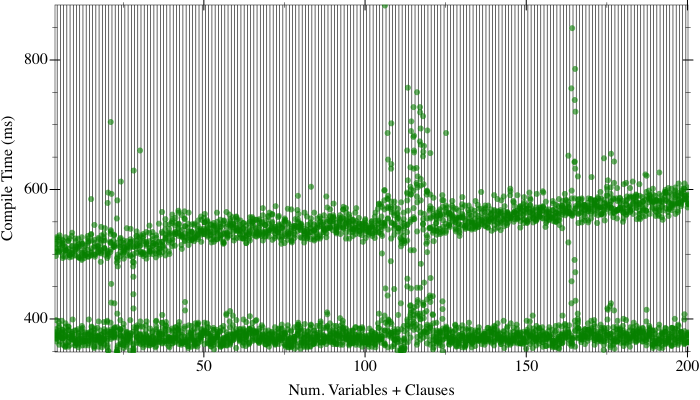
\includegraphics[width=10cm]{benchmark.png}
  \caption{Compile time vs. problem size}
  \label{fig:bench}
\end{figure}


\newpage
\section{Future Work}
\label{sec:future}

In order of importance:
\begin{itemize}
\item Connect to a third-party SAT solver
\item Implement translations for the relational operators and first-order quanitifiers
\item Benchmark large examples against Kodkod and Rosette+Z3 (sudoku solver, etc)
\item Build more a programming language for the front-end (currently need to write out large specifications ``by hand'')
\item Add symmetry detection and skolemization
\item Add minimal core extraction
\item Integrate the finished solver with Rosette
\item Use any relevant technology to improve Rosette (i.e., a better way to call external programs than with Unix pipes)
\end{itemize}


\newpage
%\section{Appendix}
\label{sec:appendix}

\subsection{Benchmark Script}

The script used to generate the plot and timings from \secref{sec:eval} is printed below.
For numbers {\tt N} between {\tt MIN-VARS} and {\tt MAX-VARS} we generate {\tt NUM-ITERS}
 random Kodkod programs with:
\begin{itemize}
\item A universe of {\tt N} atoms
\item {\tt N} relational variables, each with randomly chosen (valid) lower and upper bounds
\item {\tt N} binary propositional formulas
\end{itemize}

Time taken is measured as the real time to complete a system call that compiles
 the Kodkod program.


\begin{lstlisting}
#lang racket/base
(random-seed 8)
(require plot/no-gui racket/list racket/system racket/port)

(define NUM-ITERS 20)
(define MIN-VARS   4)
(define MAX-VARS  200)
(define TMP "kk.rkt")

(define BINOP* `(⊆ = ∧ ∨ ⇒ ⇔ ))
(define UNOP* `(no lone one some))

(define (random-ref x*)
  (list-ref x* (random (length x*))))

(define (random-slice x*)
  (define L (length x*))
  (cond
   [(< L 2) `()]
   [else
    (define lo (+ 1 (random (- L 1))))
    (define hi (random lo L))
    (take (drop x* lo) (- hi lo))]))

(define (test-random-problem n)
  (define U* (for/list ([i (in-range n)]) (format "a~a" i)))
  (define B* (for/list ([i (in-range n)])
               (define u (random-slice U*))
               (list (format "var~a" i)
                     (map list (random-slice u))
                     (map list (random-slice U*)))))
  (define F* (for/list ([i (in-range n)])
               (define op (random-ref BINOP*))
               (define u0 (random-ref UNOP*))
               (define u1 (random-ref UNOP*))
               (define v0 (car (random-ref B*)))
               (define v1 (car (random-ref B*)))
               (define expr? (memq op `(⊆ = )))
               (list (if expr? v0 (list u0 v0))
                     op
                     (if expr? v1 (list u1 v1)))))
  (with-output-to-file TMP #:exists `replace
    (lambda ()
      (displayln "#lang kodkod")
      (displayln U*)
      (for-each displayln B*)
      (for-each displayln F*)))
  (define-values (r* cpu real gc) (time-apply (lambda () (system (format "raco make ~a" TMP))) `()))
  real)

;; N = max number of variables
(define (main)
  (parameterize ([plot-font-size 16])
    (plot-file
      (append
        (for/list ([N (in-range MIN-VARS (+ 1 MAX-VARS))])
          (vrule (- N 0.5) #:width 0.6 #:color 0))
        (for/list ([N (in-range MIN-VARS (+ 1 MAX-VARS))])
          (printf "Testing ~a variables\n" N)
          (points
            (for*/list ([i (in-range NUM-ITERS)])
              (list N (test-random-problem N)))
            #:color 2
            #:alpha 0.6
            #:sym `fullcircle
            #:size 6
            #:x-jitter 0.4)))
      "output.png"
      `png
      #:x-label "Num. Variables + Clauses"
      #:y-label "Compile Time (ms)"
      #:width 700
      #:height 400)))

(module+ main
  (main)
)
\end{lstlisting}


\bibliographystyle{plain}
\bibliography{cs7485}

\end{document}
